\section{Introduction}
\label{introduction}



%%%%%%%%%%%%%%%%%%%%%%%%%%%%%%%%%%%%%%%%%%%%%%%%%%%%%%%%%%%%%%%%%%%%%%
%%%%%%%% Figure 1
%%%%%%%%%%%%%%%%%%%%%%%%%%%%%%%%%%%%%%%%%%%%%%%%%%%%%%%%%%%%%%%%%%%%%%

\begin{figure}[t]
\begin{center}
% \fbox{\rule{0pt}{2in} \rule{0.9\linewidth}{0pt}}
   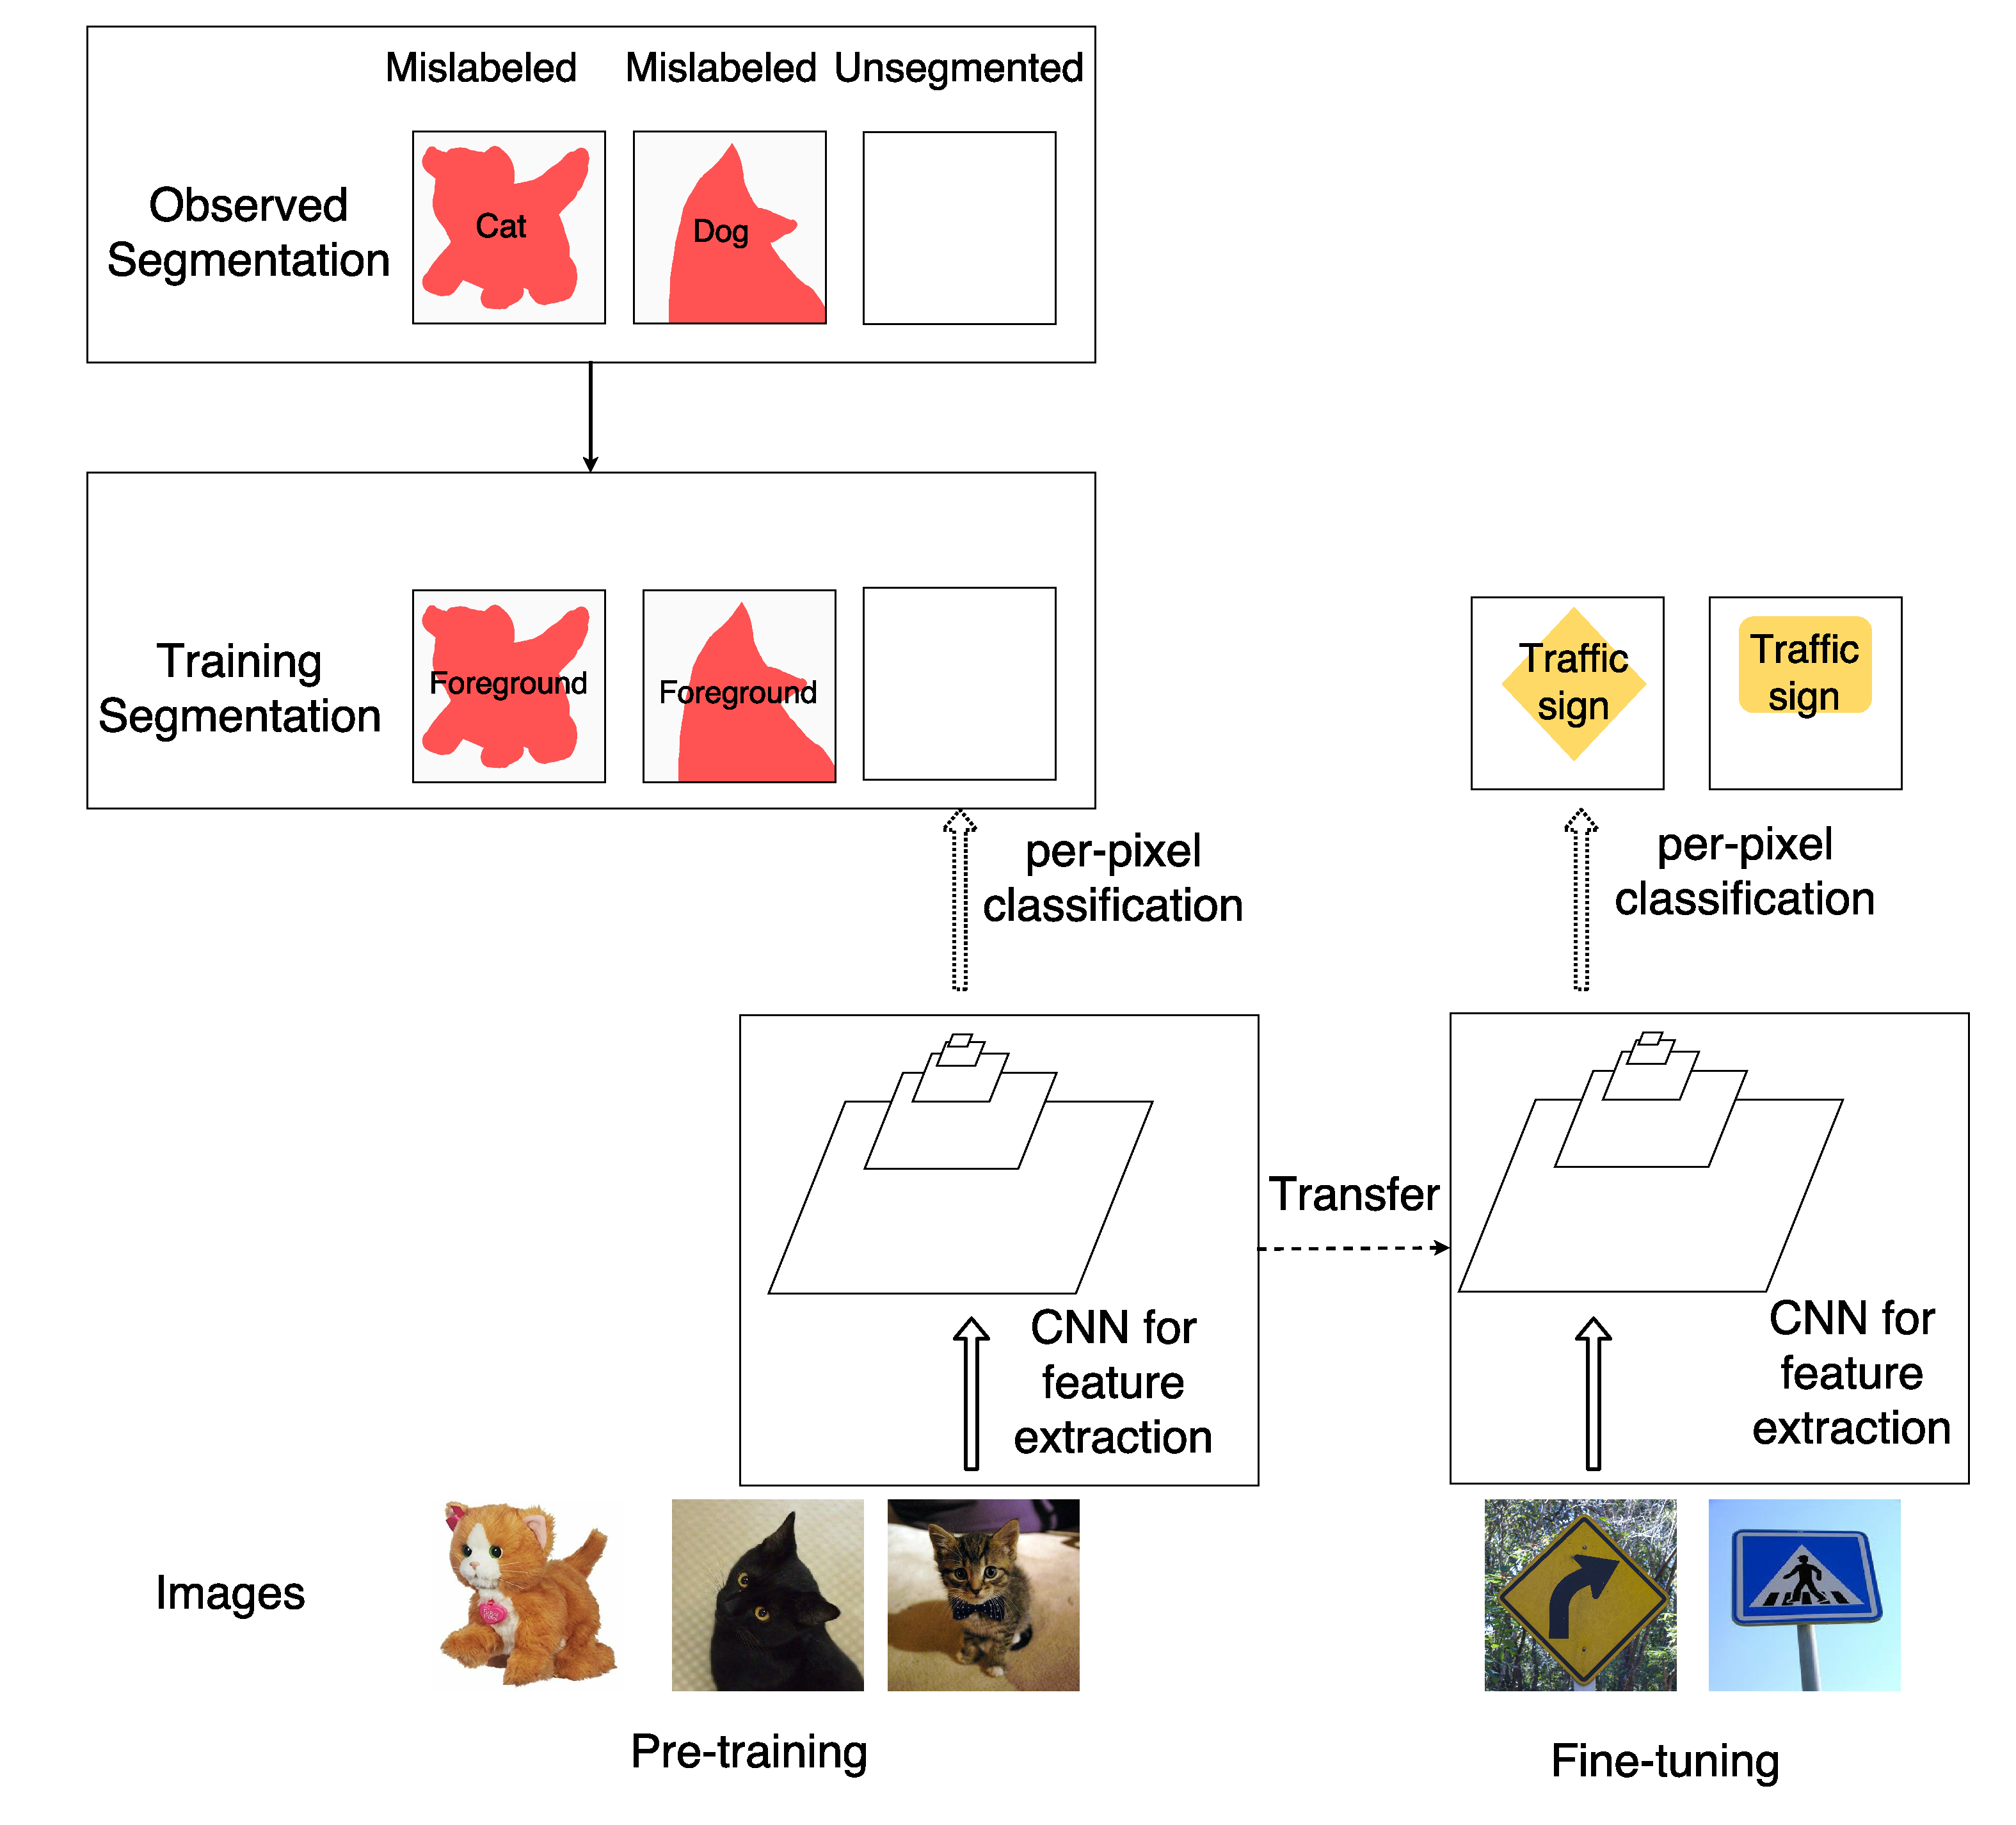
\includegraphics[width=1.0\linewidth]{img/figure1}
\end{center}
   \caption{
   Learning representations with segmentation datasets that potentially contains mislabeled objects and missing segmentation.
   The observed segmentations may contain mislabeled segments and unsegmented objects.
   We propose (1) to train foreground/background segmentation instead of per class segmentation, (2) to apply a sigmoid loss for the background class in the presence of unsegmented objects.
   The learned representations can be used as weights initialization for another dataset of interest, e.g., traffic sign segmentation.
   }
\label{fig:figure1}
\end{figure}


%%%%%%%%%%%%%%%%%%%%%%%%%%%%%%%%%%%%%%%%%%%%%%%%%%%%%%%%%%%%%%%%%%%%%%
%%%%%%%% TEXT Why transfer learning?
%%%%%%%%%%%%%%%%%%%%%%%%%%%%%%%%%%%%%%%%%%%%%%%%%%%%%%%%%%%%%%%%%%%%%%

% \noindent \textit{Why transfer learning? \\
% Segmentation model benefits from transfer learning.
% \begin{itemize}
%   \item Success of CNN benefits from large-scale data whereas segmentation datasets are small
%   \item Collecting segmentation in one domain on a large scale can be difficult.
%   \item One can transfer pre-trained CNN model to train with limited training samples access.
% \end{itemize}
% }

The often limited availability of training samples motivates most state-or-the-art deep learning based segmentation models \cite{long2015fully,chen2016deeplab,he2017mask} to transfer convolutional neural network (CNN) models \cite{krizhevsky2012imagenet,simonyan2014very,szegedy2015going,he2016deep} trained on a subset of images from ImageNet.
% The pre-trained models \cite{krizhevsky2012imagenet,simonyan2014very,szegedy2015going,he2016deep} are normally trained on an object recognition task, the ILSVRC \cite{russakovsky2015imagenet} challenge, using around 1.2 million labeled images.
% Compared to object recognition tasks, it is tougher to collect a dataset for semantic segmentation on a large scale.
The difficulty of obtaining manual segmentations is natural because it costs much more efforts for people to segment than to classify an image.
One of the largest segmentation datasets, Microsoft COCO2014 \cite{lin2014microsoft}, contains 123,287 images of 80 object categories.
As a comparison, a well-known successful task for convolutional neural networks, object recognition on the ILSRVC dataset\cite{russakovsky2015imagenet}, has around 1.2 million images for 1000 categories to train.
% the Pascal VOC2012 challenge \cite{everingham2015pascal} provides a segmentation dataset with only 9,993 segmented images for 20 object categories;
% The PASCAL-context Dataset \cite{mottaghi2014role} enriches the PASCAL VOC dataset by segmenting all 11,530 training images for 540 categories;
Transferring weights from the pre-trained ImageNet models can provide a segmentation performance boost in the limitation of lacking training samples, as reported in \cite{long2015fully} and adopted by \cite{chen2016deeplab,he2017mask}.
But the pre-trained ImageNet models are originally designed for object recognition problems, which can cause more problems than it solves.

%%%%%%%%%%%%%%%%%%%%%%%%%%%%%%%%%%%%%%%%%%%%%%%%%%%%%%%%%%%%%%%%%%%%%%
%%%%%%%% TEXT Why pre-training with segmentation?
%%%%%%%%%%%%%%%%%%%%%%%%%%%%%%%%%%%%%%%%%%%%%%%%%%%%%%%%%%%%%%%%%%%%%%

% \noindent \textit{Why pre-training with segmentation? \\
% ImageNet models have limitations.
% \begin{itemize}
%   \item Disimilarity in domain of interest for training images
%   \item Architecture limitation of ImageNet models. (3D ConvNet)
% \end{itemize}
% }

In practice, it can be challenging to employ representations from the ImageNet CNN models directly for segmentation.
Firstly, the object recognition models pursue features invariance to better capture semantics regardless the variations in objects.
The result translation invariant and resolution-reduced features reduce the localization accuracy which is not essential for object recognition but is critical for object segmentation. \cite{zheng2015conditional,chen2016deeplab}
Secondly, the ImageNet models were originally trained with natural images at relatively low resolution.
However, images to be segmented may (1) have a third dimension (3D images like CT scans and MRI scans), (2) contain extra channels (RGB-D images),  (3) be non-natural, such as aerial images and medical images.
These issues prevent transferring representations of the ImageNet models from improving segmentation performance significantly.
In this case, it can be beneficial to retrain the pre-trained ImageNet models with segmentation datasets for fine-grained cues about boundaries in the domain.

% \footnote{The KITTI Vision Benchmark Suite http://www.cvlibs.net/datasets/kitti/}

%%%%%%%% ? Deeplab https://arxiv.org/pdf/1606.00915.pdf
%%%%%%%% In particular we consider three challenges in the application of DCNNs to semantic image segmentation: (1) reduced feature resolution, (2) existence of objects at multiple scales, and (3) reduced localization accuracy due to DCNN invariance.
%%%%%%%% ? CRFasRNN http://www.robots.ox.ac.uk/~szheng/papers/CRFasRNN.pdf
%%%%%%%% Firstly, traditionalCNNs have convolutional filters with large receptivefields and hence produce coarse outputs when restructured to produce pixel-level labels [37]
%%%%%%%% Secondly, CNNs lack smoothness constraints that encourage label agreement between similar pixels, and spatial and appearance consistency of the labelling output


%%%%%%%%%%%%%%%%%%%%%%%%%%%%%%%%%%%%%%%%%%%%%%%%%%%%%%%%%%%%%%%%%%%%%%
%%%%%%%% TEXT Why labels are noisy?
%%%%%%%%%%%%%%%%%%%%%%%%%%%%%%%%%%%%%%%%%%%%%%%%%%%%%%%%%%%%%%%%%%%%%%

% \noindent
% \textit{Why labels are noisy?
% \begin{itemize}
%   \item Crowd-sourcing data is noisy by nature.
%   \item ``gold standard'' itself can be ambiguous.
%   \item There exists free available noisy segmentation datasets
% \end{itemize}
% }

The segmentation datasets for pre-training representations may contain label errors.
The use of the crowd-sourcing platform like Mechanical Turk is common nowadays to collect annotations on a large-scale.
It is natural for crowd-sourcing workers to make mistakes as a result of lack of expertise, inherent ambiguity of tasks or unconscious bias.
Enormous efforts are required, according to  \cite{lin2014microsoft,everingham2015pascal}, to ensure the correctness of segmentations.
%A slight decrease in the percentage of segmentation errors, such as from 1\% to 0\%, may require extraordinary extra efforts due to the difficulty of identifying errors.
% If not requiring ``gold standard'' segmentations for training, the efforts saved for correctness can be made to segment more images for a larger dataset.
%In some domains, for example, medical imaging, the ``gold standard'' itself can be ambiguous and cause disagreements among experts.
In addition, automated labels other than the manual ones may be freely available for particular tasks.
For example, segmentations of road and buildings for aerial images can be derived from digital maps, like OpenStreetMap, by aligning images to maps.
However, segmentations constructed in this way suffer from incompleteness as well as registration problems \cite{mnih2012learning}.
% Besides, Pl@ntNet\footnote{https://identify.plantnet-project.org/}, a crowdsourcing platform, provide millions of images of plants and corresponding labels which may or may not be correct.
Ideally, label errors in segmentations should not significantly affect the learned representations and its transferability to other datasets.

%%%%%%%%%%%%%%%%%%%%%%%%%%%%%%%%%%%%%%%%%%%%%%%%%%%%%%%%%%%%%%%%%%%%%%
%%%%%%%% TEXT What types of noises exist and motivate them?
%%%%%%%%%%%%%%%%%%%%%%%%%%%%%%%%%%%%%%%%%%%%%%%%%%%%%%%%%%%%%%%%%%%%%%

% \noindent \textit{What types of noises exist and motivate them?
% \begin{itemize}
%   \item Inexaustive segmentation
%   \item Misclassification
%   \item False segmentations
% \end{itemize}
% }

% \paragraph{Segmentation noises}

Label errors of different kinds can exist in segmentation labels.
We consider mislabelling errors occurred to the whole segment instead of individual pixels, assuming the outline of objects is always correct.
This is based on the observations that most objects in natural images have visually clear borders, and it may be untrue in some cases, for example, context segmentations\cite{mottaghi2014role}.
In particular, we consider three types of label errors: inexhaustive segmentation, objects mislabelling, and false positive segmentations.
\textbf{Objects mislabelling} from one category to another exist occasionally even for well-annotated datasets.
For example, the Microsoft COCO dataset \cite{lin2014microsoft} contains some mislabeled cats and dogs even though annotators were asked to segment only one category at a time;
\textbf{Inexhaustive segmentation} means that there exist objects left unsegmented.
A typical scenario where incomplete segmentation emerges is to segment images containing massive amounts of objects of the same kind, e.g., a flock of sheep or a pile of products;
\textbf{False positive segmentation} denotes that semantically meaningful objects from an undefined category are wrongly segmented, as objects of interest.
For instance, a dataset may contain segmentations for toy cats, labeled cats, given that toy is not one of the categories of interest and cat is.
We report in this work that objects mislabelling and inexhaustive segmentation both have a negative influence on the learned representations, whereas the false positive segmentation has little effects.


%%%%%%%%%%%%%%%%%%%%%%%%%%%%%%%%%%%%%%%%%%%%%%%%%%%%%%%%%%%%%%%%%%%%%%
%%%%%%%% TEXT Why binarizing classes?
%%%%%%%%%%%%%%%%%%%%%%%%%%%%%%%%%%%%%%%%%%%%%%%%%%%%%%%%%%%%%%%%%%%%%%

% But since label noises were proved to result in worse classificatin performance \cite{sukhbaatar2014training,patrini2016making}, it could also negatively influence the model transferability.

% \noindent \textit{Why binarizing classes?}

If negative influences to the learned representations introduced by label noises are remarkable, methods to compensate the errors become necessary.
To overcome the negative influence of objects mislabelling, we propose to group all object categories into one foreground class and train representations by learning to segment foreground and background.
Incorrect foreground labels can be considered as precise but inaccurate measurements of object class, whereas the label ``foreground'' is accurate but imprecise for segmented objects.
Grouping object categories can be regarded as converting precise but potentially inaccurate labels to accurate but imprecise labels.
We argue that learning representations do not require as precise supervision as learning classifiers.
As a matter of fact, how well the learned representations transfer to another dataset is inversely correlated to its dependence of specific categories \cite{yosinski2014transferable}.
In addition, Jain et al. \cite{jain2017pixel} demonstrated a fully convolutional network trained on over one million images to for binary segmentation generalizes well to thousands of unseen object categories.
This observation indicates that a convolutional network can learn generic knowledge about object boundaries if it can segment foreground and background for a wide range of categories sufficiently well.
Therefore, we propose to learn representations by foreground/background segmentation instead of per-class segmentation.



% Deprecated examples
% There are a few examples proved the possibility of training binary object detection/segmentation:
% Ren et al. \cite{ren2015faster} trained CNN model to perform binary classification for region of interest proposals;
% He et al. \cite{he2017mask} trained binary segmentation in addition to object detection for instance-aware segmentation;

%%%%%%%%%%%%%%%%%%%%%%%%%%%%%%%%%%%%%%%%%%%%%%%%%%%%%%%%%%%%%%%%%%%%%%
%%%%%%%% TEXT Why PU learning
%%%%%%%%%%%%%%%%%%%%%%%%%%%%%%%%%%%%%%%%%%%%%%%%%%%%%%%%%%%%%%%%%%%%%%

If we consider datasets contained missing segmentations, the problem becomes similar to a so-called \textit{positive and unlabelled learning} (PU learning) setup \cite{li2005learning}.
In the positive and unlabeled learning setup, the training dataset has two sets of examples: a \textit{positive (P) set}, containing only positive examples, and an \textit{unlabeled (U) set}, containing a mix of positive or negative examples.
% The main characteristic of the U set is no easy way to generate reliable negative labels out of it.
Semi-supervised learning techniques are not applicable in this scenario as a result of the absence of negative training samples.
The set of background pixels mixed with unsegmented object pixels, in general, fulfills this property.
In an incompletely segmented dataset, pixels of the segmented objects form the P set, and the rest pixels construct the U set.
Training with a segmentation dataset with incomplete segmentations is therefore similar to a learning problem with only positive examples and unlabeled examples.
In this work, we treat the unlabeled set as a set of examples with noisy negative labels and propose to use the sigmoid loss for the negative class.

% \noindent

% Experiments in Section \ref{subsec:robustness} indicates that inexhaustive segmentation can have significant negative influences on feature transferability.
% Besides, including mis-segmented objects for training can aggravate the inexhaustive segmentation problem.
% For example, the existence a mis-segmented toy dog does not mean that every toy dogs are mis-segmented.
% The other unsegmented toy dogs then become a source of inexhaustive segmentation and lead to worse fine-tuning performance as we discovered in Section \ref{sec:experiments}.
% Method to compensate inexhaustive segmentation is therefore necessary to train better transferable representation.

%%%%%%%%%%%%%%%%%%%%%%%%%%%%%%%%%%%%%%%%%%%%%%%%%%%%%%%%%%%%%%%%%%%%%%
%%%%%%%% TEXT Main contributions
%%%%%%%%%%%%%%%%%%%%%%%%%%%%%%%%%%%%%%%%%%%%%%%%%%%%%%%%%%%%%%%%%%%%%%

To summarize, the main contributions of this work are:
\begin{enumerate}
  \item Apart from the negative influence on classification accuracy, we present that label errors also have negative influences on the learned representations.
  \item We propose to learn representations by training foreground/background segmentations instead of by training per-class segmentation.
  \item We propose a class-dependent sigmoid loss to train deep neural networks with only positive and unlabeled data.
\end{enumerate}

%%%%%%%%%%%%%%%%%%%%%%%%%%%%%%%%%%%%%%%%%%%%%%%%%%%%%%%%%%%%%%%%%%%%%%
%%%%%%%% TEXT Table of contents
%%%%%%%%%%%%%%%%%%%%%%%%%%%%%%%%%%%%%%%%%%%%%%%%%%%%%%%%%%%%%%%%%%%%%%

The rest of this thesis is organized as follows:
In the next section, we summarize related works.
 % in areas of transfer learning, deep learning with noisy labels and PU learning.
In Section \ref{sec:formulation}, we formulate the model for segmentation model and learning with positive and unlabeled data.
The proposed sigmoid loss is evaluated, compared to the class-weighted loss, for classification with positive and unlabeled data and segmentation with positive and unlabeled data in Section \ref{subsec:pulearning} and Section \ref{subsec:incomplete} respectively.
We introduce the class-dependent, sigmoid loss for the negative class for deep learning with positive and unlabeled examples in Section \ref{sec:pulearning}.
Experiments in Section \ref{subsec:robustness} are designed to investigate the influences of objects mislabeling, inexhaustive segmentations, and false positive segmentations independently, and validate whether our proposed methods can alleviate the negative influences.
Discussions are presented in Section \ref{sec:discussion} and conclusions are summarized in Section \ref{sec:conclusion}.
%Features learned by predicting the pixel objectness with inexaustive annotations were then validated with experiments described in Section \ref{sec:discussion}.
